\section{Scraper}\label{sec:scraper}

This is the application that downloads data from the configured sources (Binance
and Coinbase).

The \code{net} package contains the classes used to call the sources' API\@. It
uses the \code{Retrofit} library to build the HTTP requests. The API responds
with JSON documents that are deserialized using the \code{Gson} library.

The main work is done by the \code{Worker} class: the scraper starts a thread
for each source and each of these threads cycles over all the markets configured
for its data source to download the market data.

The scraper also listen on a socket in order to get commands from the server
application that instruct the scraper to restart itself (and reload the
configuration from the database). This happens every time the administrator
changes the configuration for a source or a market.

\begin{landscape}
	\begin{figure}[!ht]
		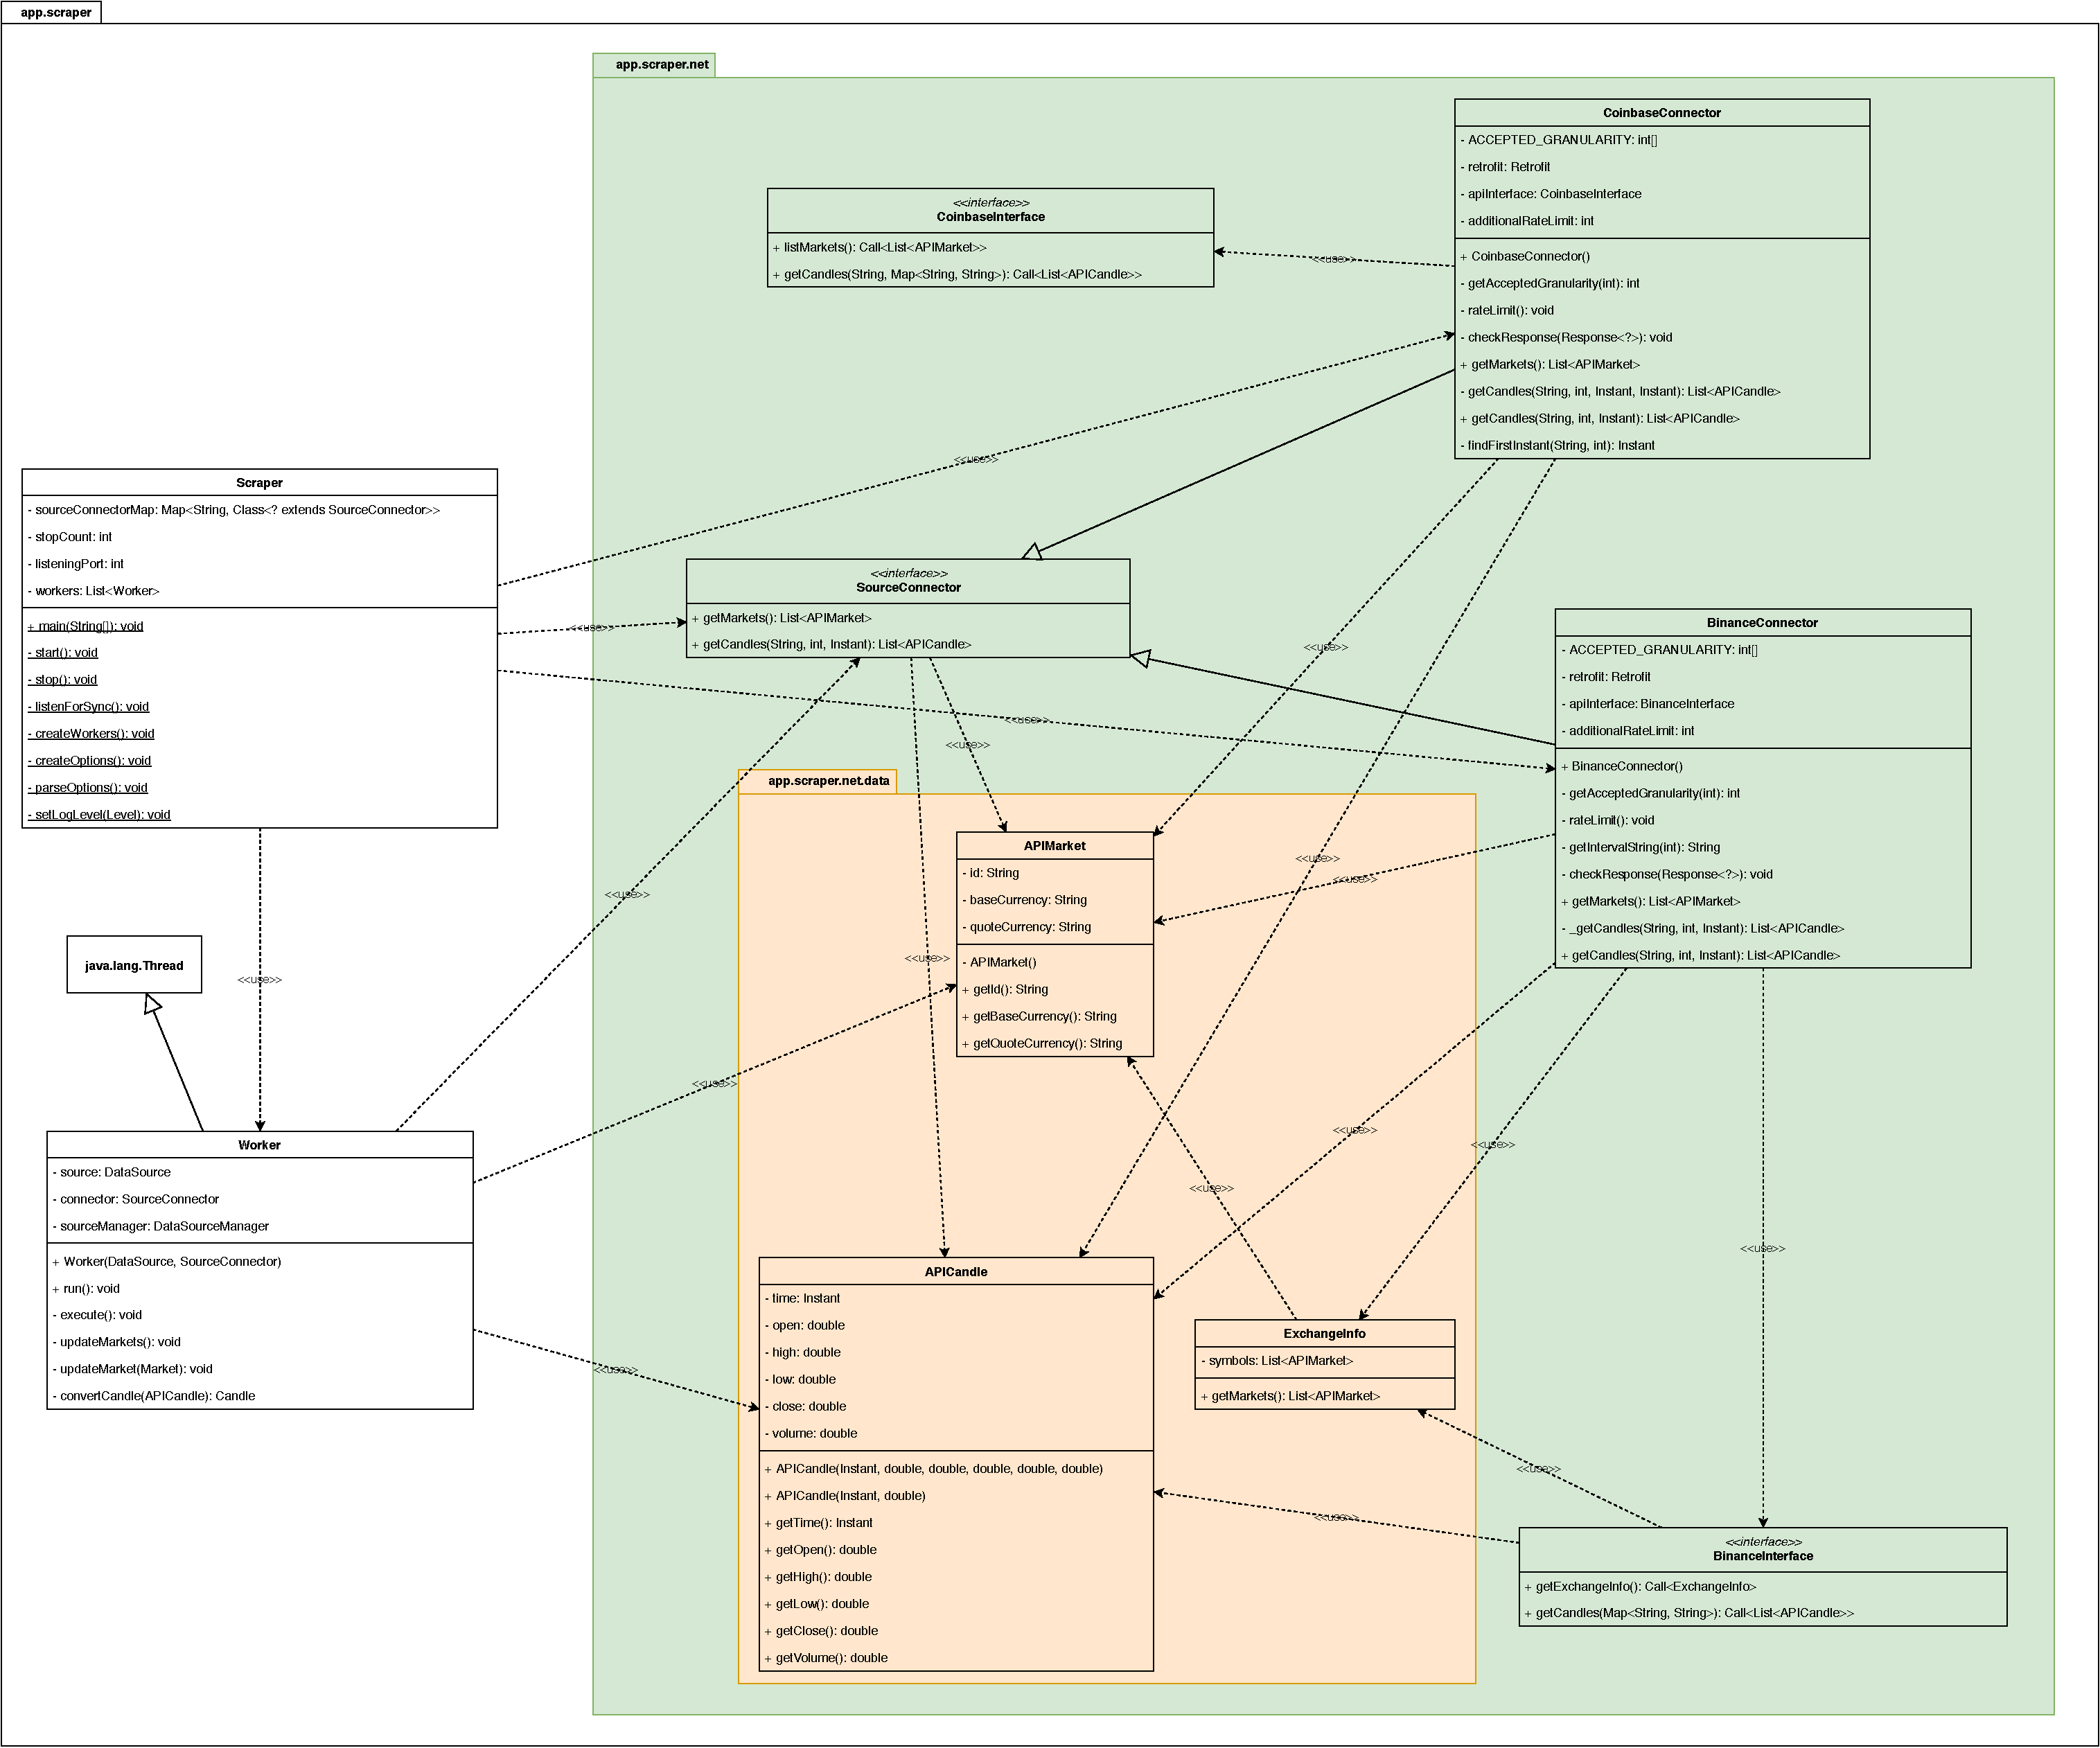
\includegraphics[width=0.7\paperheight]{module-scraper}
		\caption*{\textbf{Figure~\ref{fig:scraper}}}
		\captionlistentry{}\label{fig:scraper}
	\end{figure}
\end{landscape}
